\providecommand{\main}{..}
\documentclass[\main/tesi.tex]{subfiles}
\begin{document}
\chapter*{Introduzione} %Magari Requisiti?
\addcontentsline{toc}{chapter}{Introduzione}

L'azienda è impegnata da mesi nella creazione della seconda versione dei suoi due principali software, BrainQuick (per l'acquisizione e visualizzazione di dati encefalografici) e File Manager (un gestionale dei dati dei pazienti).\\
Una delle principali feature pianificata per l'aggiornamento di entrambi i software è le gestione centralizzata dei dati, in particolare le impostazioni e i cosiddetti "montaggi", ossia dei file descrittivi dei tracciati EEG acquisiti.\\
Viene richiesto che le impostazioni (chiamati dall'azienda anche \textit{settaggi}, che sarà la forma con la quale saranno chiamati per il resto del documento) siano sincronizzabili tra i dispositivi in 4 diversi \textit{scope}, ossia un identificatore rispetto a quale tipo di entità è associato ogni settaggio.\\
Gli scope sono
\begin{itemize}
    \item \textbf{Sistema}: I valori dei settaggi con questo scope condivisi tra tutti gli utenti e unità (macchine fisiche).
    \item \textbf{Utente}: I valori dei settaggi con questo scope sono legati al singolo utente, idipendentemente dall'unità.
    \item \textbf{Unità}: I valori settaggi con questo scope sono legati alla singola unità.
    \item \textbf{Utente ed Unità}: I settaggi con questo scope sono legati ad un singolo utente accoppiato ad una specifica macchina.
\end{itemize}
La soluzione che si intende modellare deve seguire determinati requisiti e possedere specifiche capacità, oltre a dei generali principi di progettazione da seguire per un software di alta qualità.

\section{Situatione iniziale e compatibilità}
BrainQuick e FileManager sono entrambi software sviluppati con il framework .NET \cite{dotnet} in C\# \cite{csharp}.\\
Questi software fanno già largamente utilizzo di un sistema di impostazioni basato sui file ".ini", semplici file di testo che seguono una certa codifica, nei quali salvano e dai quali caricano i valori dei settaggi.\\
È un sistema molto semplice e limitato e di conseguenza inutilizzabile ai fini di una centralizzazione dei dati.\\

Altri dati non considerabili come impostazioni del software ma piuttosto dei dati di supporto per il funzionamento, ad esempio i montaggi precedentemente citati, vengono salvati in file dedicati in formato XML \cite{xml}.\\
A livello implementativo, i dati sono ottenuti attraverso una classe singleton \textbf{SettingsService} che con un apposito metodo restituisce un'istanza di una classe \textit{contenitore} di una serie di settaggi.\\
È quindi impossibile ottenere direttamente un singolo settaggio, bisogna prima ottenere il contenitore che lo contiene.\\
In sostanza ogni classe contenitore definisce una serie di settaggi che poi vengono serializzati con il metodo \textbf{SetSetting} e deserializzati con \textbf{GetSetting}.

\section{Tipi di dati supportati}
È necessario supportare tutti i principali tipi primitivi di rappresentazione numerica, intera o a virgola mobile, comunemente usati nei linguaggi di programmazione.\\
In questo caso:
\begin{itemize}
    \item \textbf{Byte, short, int, long}.
    \item \textbf{Single, float, double, decimal} (quest'ultimo è un numero a virgola mobile a 128 bit).
\end{itemize}
È inoltre richiesto il supporto ad alcune semplici strutture dati rappresentati dati comuni, quali:
\begin{itemize}
    \item \textbf{DateTime} per la rappresentazione di un momento nel tempo con precisione fino ai millisecondi.
    \item \textbf{TimeSpan} per la rappresentazione di una quantità di tempo trascorso sempre preciso al millisecondo.
\end{itemize}
I tipi di dato citati in precedenza devono essere supportati anche in gruppi, rappresentati come vettori e da gestire sotto forma di blocco unico (non è richiesto quindi che ogni valore del vettore sia modificabile o sincronizzabile singolaramente).\\
Possono inoltre essere rappresentati sotto forma di stringhe (funzionalità necessaria per il salvataggio) seguendo gli standard del linguaggio.\\

Per quanto riguarda oggetti complessi, come ad esempio i montaggi, si necessita siano supportati sia singolarmente, che in vettori di lunghezza non fissa, che potranno anche modificare la loro dimensione in caso sia necessario.\\
Ogni oggetto appartenete ad un vettore deve quindi essere aggiungibile, modificabile, salvabile e sincronizzabile singolaramente rispetto agli altri del vettore di cui fa parte.\\
I vari settaggi devono essere poi raggruppabili all'interno di classi, che non influiscono però sul processo di salvataggio/recupero dei dati, ma esistono solo a livello di utilizzo nel codice per una maggiore chiarezza (esattamente come i "gruppi" citati in precedenza).\\
L'unica differenza sostanziale a livello di supporto dati rispetto al sistema precedente basato sui file ini è la possibilità di gestire singolarmente i valori nei vettori.

\section{Inizializzazione}
Il salvataggio di questi settaggi è richiesto avvenga attraverso database relazionali, sia nel caso del salvataggio locale che nel caso del salvataggio remoto.\\
La presenza quindi di un database centrale e multipli database locali (uno per ciascun client in cui viene installato il software) introduce la necessità di inizializzarli ad un preciso schema relazionale prima che possano essere utilizzabili e di conseguenza abilitare la centralizzazione.\\
Mentre è stato deciso che il database locale avrebbe seguito la strada più ovvia, ossia essere creato, inizializzato ed eventualmente aggiornato dal programma stesso al primo avvio, quello centrale ha richiesto una scelta a livello di politica aziendale sulla base degli strumenti hardware e software forniti dai clienti finali (tipicamente ospedali).\\
Nella maggioranza dei casi, viene fornito un computer dotato di \textbf{Windows Server} \cite{windowsserver} connesso alla stessa rete locale dei computer nei quali saranno installati i software dell'azienda.\\
Per quanto riguarda l'installazione del DBMS, può essere effettuata manualmente, ma per la creazione dell'effettivo database e il suo popolamento quando necessario si sono valutate due soluzioni:
\begin{itemize}
    \item Un programma di utility (che non richieda installazione) che si occupi solo di inizializzazione e aggiornamento del database.\\Sarebbe da utilizzare manualmente e solo in caso di necessità, come la prima installazione o eventuali aggiornamenti.
    \item Un vero e proprio programma di backend web che faccia da livello di astrazione tra il database centrale e i programmi installati nei singoli computer, attraverso richieste HTTP (ad esempio \textbf{REST} \cite{rest}).\\Si tratta di una scelta più onerosa in quanto aumenterebbero i software da sviluppare, ma ridurrebbe parte del peso computazionale (ad esempio calcolare la differenza tra settaggi locali e remoti durante la sincronizzazione) che altrimenti sarebbe svolto dai singoli client e faciliterebbe una possibile futura migrazione a piattaforme cloud.
\end{itemize}
Nonostante la seconda opzione sia stata considerata la migliore a lungo termine, la mancanza di tempo e l'incertezza sulle eventuali policy dei clienti riguardo l'installazione nei loro server di ulteriori componenti oltre al DBMS hanno spinto l'azienda a scegliere la prima, chiedendo però un'implementazione flessibile che riduca al minimo gli sforzi per eventualmente cambiare soluzione.

\section{Sincronizzazione}
Sono stati forniti i seguenti requisiti riguardo il comportamento del client (che è, viste le scelte precedenti, il software che integra la soluzione sviluppata contenente la logica di sincronizzazione) in tutti i casi supportati:
\begin{itemize}
    \item Il client deve supportare la centralizzazione ma essere in grado di funzionare anche nel caso non sia disponibile il database centrale, con l'eventuale sincronizzazione che avverrebbe alla prima riconnessione.
    \item Il client deve essere in grado di funzionare autonomamente sin dal primo avvio, nel caso il cliente scelga una soluzione non centralizzata e, nel caso cambi idea, deve essere in grado di connettersi ad una nuova istanza centralizzata.\\In questo caso i valori dei settaggi maturati fino a quel momento vengono sovrascritti con quanto presente nell'istanza centralizzata.
\end{itemize}
Inoltre, nello specifico, la sincronizzazione di un particolare settaggio avviene secondo i seguenti requisiti:
\begin{itemize}
    \item nel caso il settaggio remoto sia stato modificato dopo l'ultima sincronizzazione con il client, viene aggiornato il database locale con il nuovo valore.
    \item Nel caso il settaggio locale sia stato modificato dopo l'ultima sincronizzazione con il database centrale, viene aggiornato il database centrale con il nuovo valore. 
    \item Nel caso sia il settaggio remoto che quello locale siano stati aggiornati successivamente all'ultima sincronizzazione tra i due database (da ora in poi questa situazione sarà chiamata \textbf{conflitto}), il nuovo valore del settaggio sarà quello del settaggio aggiornato più di recente.
    \item Nel caso avvenga un conflitto e il settaggio remoto abbia una policy collegata (di cui si parlerà nella prossima sezione), allora viene scelto il valore contenuto nel database remoto.
\end{itemize}
Deve inoltre essere supportata la sincronizzazione automatica in modo che, una volta impostato un range di tempo, la sincronizzazione avvenga indipendentemente da quanto stia facendo l'utente in quel momento e che il sistema rispecchi i cambiamenti avvenuti.

\section{Le Policy}
Una feature essenziale che questo modulo introduce rispetto alla precedente implementazione è il concetto di policy.\\
Capita spesso infatti che i software vengano distribuiti in grandi ospedali che possiedono centinaia di terminali, rendendo dispendioso configurarli manualmente in caso sia necessario che i settaggi siano standardizzati tra i dispositivi.\\
Sono state quindi pensate le policy, ossia regole di importanza superiore rispetto alle decisioni del singolo client in materia di configurazione e che creano a tutti gli effetti un sistema di governabilità dei settaggi a livello centrale.\\
Una policy deve possedere le seguenti capacità:
\begin{itemize}
    \item Deve poter definire se un client possa modificare uno specifico settaggio.
    \item Deve poter sovrascrivere in qualsiasi momento i settaggi nel database centrale indipendentemente dal loro scope (i client riceveranno le modifiche alla prima sincronizzazione successiva).
    \item Deve essere raggruppabile con altre policy, in modo da poterle applicare o rimuovere in blocco.
\end{itemize}

\subsection{Il programma di gestione delle Policy}
La gestione delle Policy sarà compito del personale dell'ospedale e si deve presumere non sia personale formato a livello tecnologico.\\
Di conseguenza, si richiede venga fornita un'applicazione standalone il cui compito sia fornire una UI per una gestione semplice di tali policy.\\
Questa applicazione deve essere utilizzabile da qualsiasi client connesso alla rete locale e permettere tutte le operazioni consentite dalle policy.\\
Prima della progettazione del modulo, era già stato creato un prototipo completo a livello estetico ma senza logiche implementate.

\section{Requisiti aggiuntivi}

\subsection{Integrazione}
A livello di codice, l'integrazione deve riprendere il più possibile quanto di già esistente.\\
Si vuole quindi che l'attuale \textbf{SettingService} e la relativa interfaccia \textbf{ISettingService} siano mantenuti, anche se alcuni cambiamenti sono necessari.\\
Va infatti aggiunto il supporto al sistema di sincronizzazione, totalmente assente nelle precedenti versioni, oltre ad una serie di eventi registrabili che notifichino l'utilizzatore del modulo di eventuali errori o del completamento di una delle fasi importanti del sistema.\\
Si vuole poi aggiungere la possibilità di annullare eventuali modifiche non ancora sincronizzate, operazione che precedentemente veniva svolta semplicemente non salvando, in questo caso va eseguita manualmente per via della sincronizzazione automatica che potrebbe dare effetti inattesi.\\
Come detto in precedenza il nuovo SettingsService restituirà, esattamente come il vecchio, delle istanze di classi container degli effettivi settaggi e di conseguenza il metodo che se ne occupa potrà rimanere invariato a livello di firma.\\
Vale la pena notare che i singoli settaggi non potranno più essere inseriti nel container direttamente come valore, ma saranno necessarie delle strutture intermedie che permettano di gestire le policy, degli eventi aggiuntivi e gli aggiornamenti dei valori.

\subsection{Testing e Documentazione}
\label{testing}
I software medicali (e di conseguenza anche il modulo in oggetto, in quanto parte di altri software) devono sottostare ad uno specifico ciclo di sviluppo, definito dallo standard \textbf{IEC 62304} \cite{iec62304}.\\
Tale standard definisce le fasi alle quali deve sottostare un software medicale per essere considerato di qualità.\\
In particolare, in base alle fasi che vengono rispettate, vengono assegnate delle classificazioni dalla A alla C, dove la C è quella dedicata ai software che rispettano tutte le fasi.\\
\begin{figure}[h]
    \caption{Processo di sviluppo software secondo lo standard IEC 62304.}
    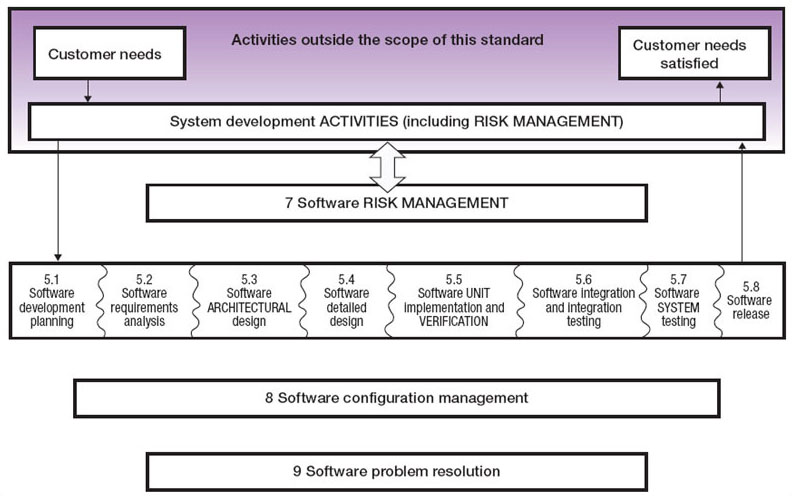
\includegraphics[width=\textwidth]{../images/quality.png}
\end{figure}
Le fasi sono (in ordine):
\begin{itemize}
    \item Pianifica dello sviluppo del software
    \item Analisi dei requisiti del software
    \item Progettazione architetturale del software
    \item Progettazione dettagliata del software
    \item Implementazione del software
    \item Verifica del software
    \item Integrazione e testing di integrazione del software
    \item Testing del sistema software
    \item Release del software
\end{itemize}
In questo documento verranno affrontati solo i passaggi che vanno dalla progettazione architetturale al testing del sistema, in quanto i requisiti (e di conseguenza le fasi precedenti) sono stati forniti in precedenza, mentre la release avverrà in futuro.\\

Nei requisiti forniti non è stata definita alcuna esigenza specifica sul testing automatico del codice, ma è stato generalmente richiesto che venisse progettata una test suite con bassa priorità rispetto al resto.\\
È stato quindi stilato un semplice piano di testing aggiuntivo ai requisiti che si concentra sullo \textit{unit testing} della sincronizzazione (dati diversi stati di partenza).\\

Per quanto riguarda la documentazione, è stato richiesto di stilare un documento utilizzando \textbf{Microsoft Word} che spieghi il funzionamento e i requisiti del modulo per poter essere integrato.\\

\end{document}